\chapter{Методика организации виртуальных экспериментов в практических задачах} \label{chapt3}

\section{Задачи по анализу сигналов фМРТ в нейрофизиологии}\label{sect_4_1}
\subsection{Введение}
Для сообщества, занимающегося нейронаукой, разработка общих парадигм исследования огромного числа функциональных систем 
в головном мозге все еще остается труднейшей задачей. Построенный на термине коннектом, изобретенном для описания 
подробной карты соединений нейронов в мозге человека, термин функциональный коннектом обозначает совокупное множество 
функциональных соединений в мозге (его схему коммутации) \cite{biswal2010toward}. В более широком смысле коннектом 
включает в себя отображение всех нейронных соединений нервной системы организма. Вопросы образования и изучения 
коннектома, известные как коннектомика, могут простираться по своему масштабу от детальной карты полного набора 
нейронов и синапсов в пределах части или всей нервной системы организма до описания макромасштабных процессов 
\cite{craddock2013imaging} функциональной и структурной межнейронной коннективности между всеми полями коры головного 
мозга и субкортикальными структурами. Конечная цель коннектомики "--- картирование мозга человека. В функциональной 
магниторезонансной томографии (fMRI "--- фМРТ) считается, что визуализируемые соединения представляют собой 
функциональную связность в том смысле, что две области мозга совместно участвуют в реализации некоторой более высокого 
порядка функции, нередко в контексте выполнения определенной задачи. 

Технология fMRI стала мощным инструментом, используемым для изучения многочисленных функциональных схем одновременно. 
Это привлекло к себе внимание статистиков, работающих в этой сфере. На уровне элементарных измерений данные 
нейровизуализации могут, в основном, рассматриваться как состоящие из ряда сигналов (как правило, последовательных во 
времени) в каждой совокупности пикселей (в двух измерениях) или вокселей (в трех измерениях). Исходя из этих данных, 
нейровизуализация использует различные формы представления информации более высокого уровня. За последние годы в 
нейровизуализации возник существенный интерес к представлениям на основе сетей, где сети (графы) используются для 
обобщения информации о связях в множестве измерений, обычно предполагающих отражение функциональных или структурных 
отношений между исследуемыми областями мозга. Нетрудно предсказать, что поскольку нейровизуализация стала теперь 
стандартным инструментом клинической нейронауки, мы быстро движемся к моменту, когда в нашем распоряжении окажутся 
доступные базы данных, состоящие из больших массивов вторичной информации в виде объектов данных на основе сетей. 

Одной из наиболее фундаментальных задач, представляющих интерес в анализе таких данных, является проверка гипотез, 
отвечающих на такие вопросы, как Есть ли разница между сетями (графами) этих двух групп объектов?. Сети не являются 
эвклидовыми объектами, и поэтому классические методы статистики здесь нельзя применять непосредственно. Аналоги 
классических инструментов оценки (на основе статистики) и проверки гипотез исследуются в 
\cite{ginestet2017hypothesis, ginestet2014statistical}. Такое исследование мотивировано проектом 1000 функциональных 
коннектомов (1000 FCP), запущенном в 2010 г. \cite{biswal2010toward}. Проект 1000 FCP \cite{yan2013standardizing} 
включает в себя самое большое множество данных такого рода, сходного с большими множествами данных в генетике. 
В проект 1000 FCP включено описание данных функциональной нейровизуализации 1093-х субъектов, находящихся в 
24 центрах сообщества. Средний возраст участников "--- 29 лет, а все субъекты были возрастом 18 лет или старше.


Другие проекты (такие как проект Коннектом человека (Human Connectome Project "--- HCP) \cite{VanEssen2013}) имеют 
целью построить сетевую карту (граф) мозга здорового, живого взрослого человека. Суммарный объем данных, выдаваемых 
проектом HCP, будет, по-видимому, составлять много петабайтов \cite{VanEssen2013}. Из информатики платформа HCP 
включает в себя как платформу систему управления данными ConnectomeDB на базе платформы визуализации XNAT из той 
же информатики \cite{marcus2007extensible}, широко используемую систему с открытым кодом для управления и совместного 
пользования данными визуализации и взаимосвязанными данными. В настоящее время проект HCP располагает информацией о 
более чем 1000 субъектам, включая структурные сканы (\textit{T1w} и \textit{T2w}), fMRI в покое (rfMRI), 
fMRI действия (tfMRI) при выполнении задачи, а также диффузионная визуализация МРТ (dMRI) с высокой угловой 
разрешающей способностью. Кроме того, доступны данные MEG в покое (rMEG) и/или данные MEG (tMEG) при выполнении задачи. 
Данные поступают в нескольких форматах: необработанные сырые данные, предварительно минимально обработанные, 
а также наборы данных по результатам анализа. В предварительно обработанных наборах данных пространственные нарушения 
минимальны, а данные были выровнены по их модальностям и по субъектам с использованием соответствующих методов 
регистрации по объемам и по поверхностям. Сообщество исполнителей проекта HCP рекомендует пользоваться 
предобработанными наборами данных. 

Можно ожидать, что в ближайшем будущем в нейронауке появится большое количество баз данных сетевых объектов, 
мотивирующих разработку и расширение различных инструментов от классической статистики до глобальных сетевых данных.

Исследование функциональной связности с помощью fMRI широко используется, так как метод обладает высоким 
пространственным разрешением, анализ проводится интактно, не требуя инъекций или хирургических вмешательств. 
Данные fMRI представляют собой 4-х мерные изображения (одна временная координата и три пространственных) и 
предназначены для регистрации гемодинамических реакций головного мозга, вызванных активностью нейронов. 
Различают два типа fMRI: 1) изображения fMRI, которые были получены, когда человек находился в состоянии 
покоя, то есть во время проведения эксперимента испытуемого просили закрыть глаза, расслабиться и ни о чем не 
думать; 2) изображения fMRI, которые были получены во время некоторого действия, например, у испытуемого 
стимулируется проявление эмоций, зрительных или двигательных реакций и пр. Изображения fMRI имеют сложную 
структуру и требуют больших ресурсов для их хранения, таких как высокопроизводительные вычислительные системы. 

% TODO типы взаимодействия
%Существует три типа взаимодействия между регионами головного мозга: структурное, эффективное и функциональное. 
Исследование функциональной связности в состоянии покоя имеет существенное значение, так как полученные результаты позволяют выделять нейросети покоя и анализировать их активность. Другим примером связности является эффективная связность. Анализ эффективной связности показателей fMRI действия позволяют оценить участие конкретных структур мозга в обеспечении сложных функций, таких как язык, память, азартная игра, движения. Эти подходы используются для изучения когнитивных и других функций мозга, а также для исследования различных заболеваний: болезни Паркинсона, синдром дефицита внимания/гиперактивности, болезни Альцгеймера и др. Задачи исследования различных типов связности являются актуальными и представляют существенный интерес.

\subsection{Выделение регионов головного мозга из fMRI изображений}

Визуализация, обработка и анализ многомерных данных, таких как изображения, часто требует некоторой предварительной обработки, для того чтобы уменьшить размерность данных и получить отображение исходно представленных данных на низкоразмерное векторное пространство. Предположение таково, что исходные данные находятся в низкоразмерном подпространстве или многообразии \cite{brun2006manifold}, вложенном в исходное пространство. Эта часть исследований называется сокращением размерности, или нелинейным сокращением размерности, включающей в себя методы параметризации данных с использованием низкоразмерных многообразий (манифольдов) в качестве моделей. В сообществе обработчиков информации по нейронам это известно под названием обучения на базе многообразий. Методы обучения на базе многообразий дают возможность отыскивать нелинейные параметризации многообразий информационных точек, находящихся в высокоразмерных пространствах, весьма сходно с тем, как метод главных компонент (МГК) способен узнавать или выявлять наиболее важное линейное подпространство набора информационных точек (проецируя данные на $n$-размерное линейное подпространство, которое дает максимум дисперсии распределения вероятностей данных в новом пространстве). Такие преобразования называются выделением регионов головного мозга человека.

В качестве переменных для построения зависимостей используются регионы головного мозга (ROI). ROI — это набор анатомически близких вокселей, которые представляют собой встроенные единицы изображения МРТ, представляющие маленькие кубики мозга. Поскольку изображение МРТ фиксирует изменения во времени уровня кислорода в крови, каждый воксель связан с соответствующим временным рядом. ROI также связаны с временными рядами, например, усредненными по всем временным рядам его вокселей. На данном этапе требуется преобразовать 4-х мерное изображение головного мозга в двухмерный массив (регионы головного мозга – время). Выделение регионов можно рассматривать как один из способов уменьшения размерности. При использовании данного подхода регионы некоторым образом группируются и усредняются, а само усредненное значение является представительным значением для данного региона. Также при использовании данного метода делается предположение, что воксели одного региона ведут себя схожим образом. 

Существует множество методов для выделения регионов головного мозга \cite{Arslan2018}. Все методы можно разделить на три группы:
\begin{enumerate}
    \item Выделение регионов для одного человека (субъекта);
    \item Выделение для группы людей;
    \item Использование различных атласов головного мозга человека.
\end{enumerate}

Методы первого типа подразделяют поверхность головного мозга каждого субъекта независимо друг от друга. Часть методов в данном подходе основа-на на широко используемых алгоритмах кластеризации, таких как $k$-средних \cite{arslan2015multi}, агломеративной иерархической кластеризации \cite{blumensath2013spatially} и спектральной кластеризации \cite{van2008normalized}. Если набор данных состоит из нескольких субъектов, то первоначально все данные объединяются в один большой набор, состоящий из $M$ субъектов, а затем применяются МГК/МНК.

При больших наборах данных или при большом количестве субъектов становится неразумным формировать полный набор данных, а затем применять МГК и МНК из-за ограничений по памяти и по вычислительному времени. Для решения этой проблемы было предложено использовать групповые методы. Групповые методы строят репрезентативные модели популяции. Методы получения регионов группового уровня обычно основываются на предположении, что пространственное соответствие между субъектами было обеспечено априори. Следовательно, каждая вершина (или воксель) представляет собой одно и то же пространственное положение для каждого субъекта. Это позволяет объединить или усреднить данные по различным субъектам для анализа на популяционном уровне. Существует два наиболее популярных способа.

Первым способом является вычисление регионов для каждого субъекта индивидуально, а затем применение второго уровня алгоритма кластеризации на уровне популяции (т. е. двухуровневый подход). Двухуровневый подход обеспечивает группировку вокселей одних и тех же регионов вместе. В результате регионы группового уровня, полученные с помощью этого метода, выражают общие характеристики популяции, аппроксимируемые регионами, полученные для каждого субъекта в отдельности. Примером является применение двухуровненого применение метода главных компонент \cite{calhoun2001method} (см. \cref{fig:two_step_pca}). Сначала каждый набор данных сокращается до $\rho$ основных пространственных векторов с использованием МГК, а затем объединив их и применив еще раз  МГК, чтобы уменьшить конечный набор данных до $k$ компонент.

\begin{figure}[ht]
    \centering
    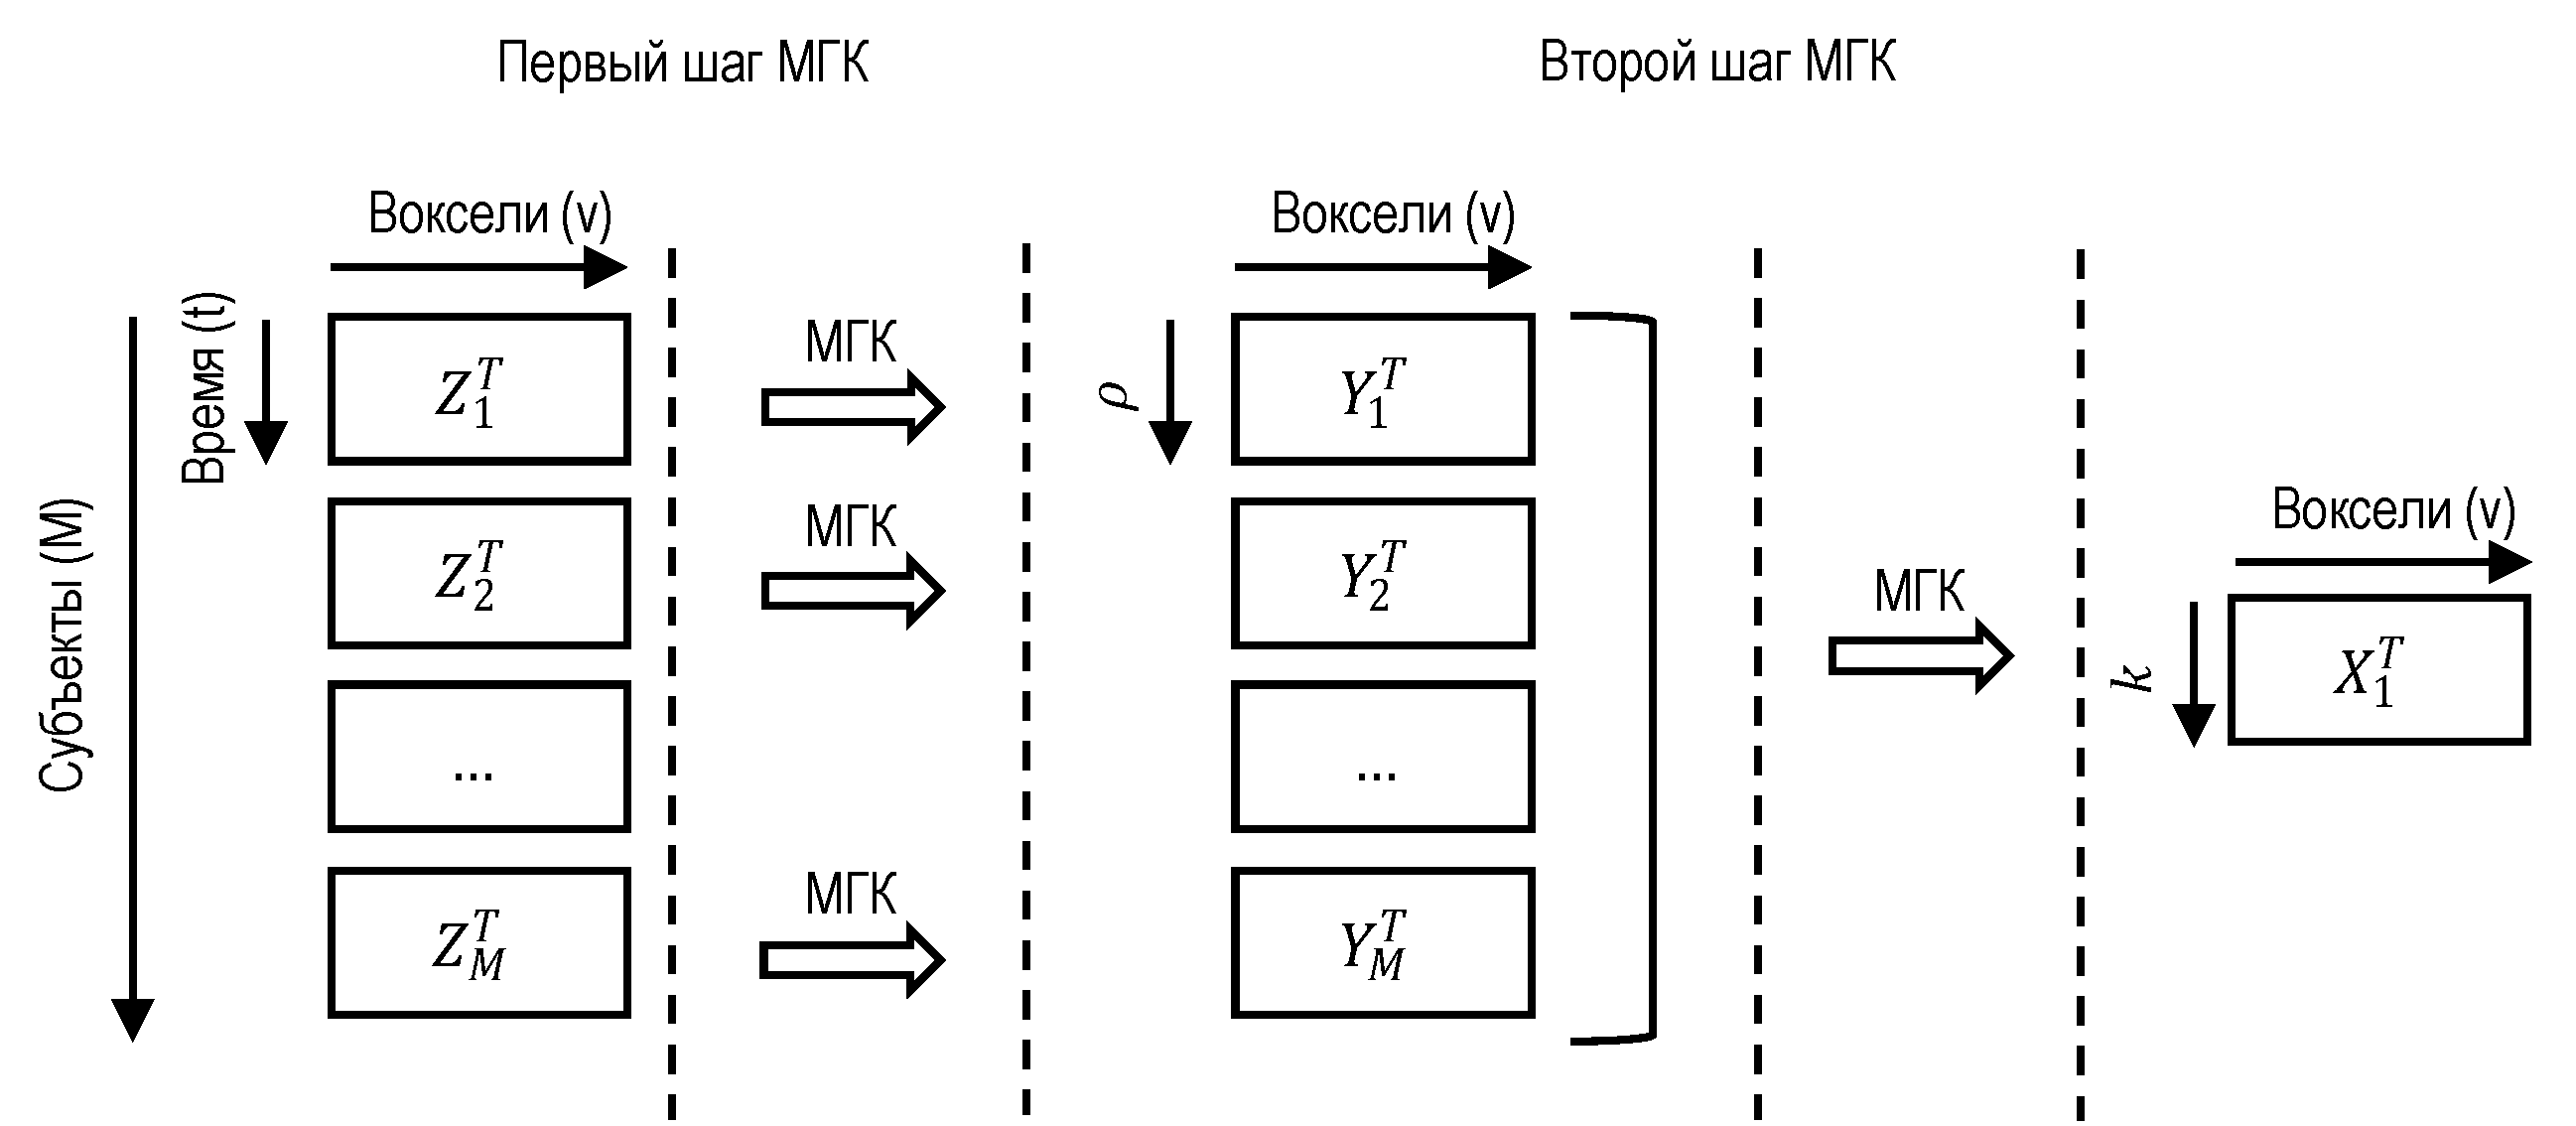
\includegraphics[width=1.0\linewidth]{images/two_step_pca.pdf}
    \caption{Двухуровненое применение метода главных компонент.}\label{fig:two_step_pca}
\end{figure}

Хотя использование небольшого значения $m$ ограничивает требования к памяти для этих операций, размер данных масштабируется линейно с количеством объектов, которые в конечном итоге могут стать непрактично большими. Кроме того, важная часть информации может быть потеряна, если $m$ не является относительно большим (обычно оно не должно быть большим). Информацию может быть трудно оценить на уровне отдельного субъекта, но она может быть важна на уровне группы. 

Вторым способом является вычисление репрезентативной матрицы признаков из популяции, например, путем объединения временных рядов и далее подходу группового среднего. Данный метод направлен на поиск общих паттернов между индивидами в пределах популяции путем вычисления группового среднего представления, что достигается путем объединения временных рядов каждого субъекта и применения метода главных компонент или его модификаций для уменьшения размерности для выделения регионов (см. \cref{fig:group_pca}). Широко используемым является алгоритм MELODIC Incremental Group-PCA (MIGP) \cite{rachakonda2016memory} . MIGP "--- это инкрементный подход, целью которого является обеспечение очень близкого приближения к полной конкатенации набора данных, за которым следует МГК, но без больших требований к памяти. Высокая точность достигается за счет того, что отдельные наборы данных субъектов не сводятся к небольшому числу компонентов МГК. Инкрементный подход сохраняет внутреннее пространство МГК из $m$ взвешенных пространственных собственных векторов, где $m$ обычно больше, чем количество временных точек в каждом отдельном наборе данных. Под "взвешенным" подразумевается, что собственные значения включены в матрицу пространственных собственных векторов. Конечный набор из $m$ компонентов, представляющих временно объединенные выходные данные МГК, затем может быть уменьшен до требуемого размера $n$ просто путем сохранения верхних $n$ компонентов и, при необходимости, отбрасывания весовых коэффициентов (собственных значений).

Обычно сначала объединяются 2-3 субъекта. Затем этот набор данных вводится в $m$-мерный объект и получается следующая матрица. Каждый вектор умножается на свое собственное значение. Собственные значения характеризуют важность компонента здесь, поэтому статистическая информация не теряется и сохраняется дисперсия каждого субъекта. MIGP не увеличивает требования к памяти с увеличением числа объектов, большие матрицы никогда не формируются, а время вычисления линейно зависит от количества объектов.

\begin{figure}[ht]
    \centering
    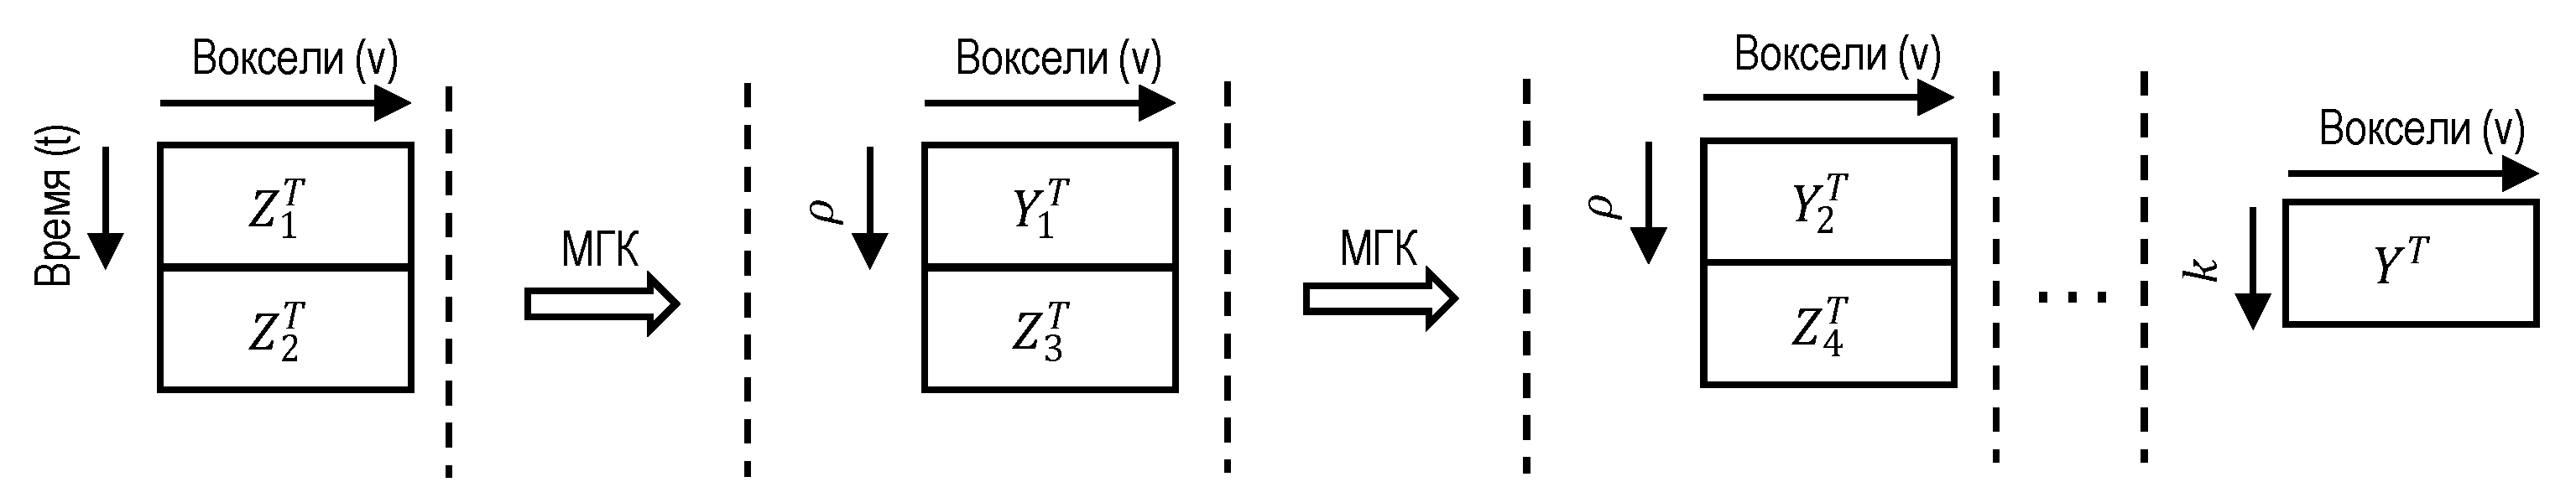
\includegraphics[width=1.0\linewidth]{images/group_pca.pdf}
    \caption{Последовательное применение метода главных компонент.}\label{fig:group_pca}
\end{figure}

При работе с атласами головного мозга человека используется заранее вычисленная функция, ставящая каждому вокселю изображения в соответствие регион головного мозга. Существует множество атласов головного мозга человека, например, вероятностный атлас Harvard-oxford \cite{desikan2006automated}, в котором описано 48 кортикальных регионов и 23 субкортикальных. В работе \cite{fischl2004automatically} проводились ряд экспериментов по результатам которых делается вывод об оптимальном количестве структурных регионов. Проведен сравнительный анализ на нескольких наборах данных между ручной разметкой и при помощи атласа Destrieux 2009. Авторы статьи утверждают, что оптимальное количество регионов в атласе 150–160, при таком количестве удаться достичь баланс между размерностью данных и качеством извлекаемого сигнала. Automated Anatomical Labeling (AAL) атлас является результатом автоматической анатомической маркировки пространственно нормализованного набора данных фМРТ высокого разрешения, предоставленного Монреальским неврологическим институтом (MNI). Данный атлас включает 116 структурных областей головного мозга \cite{tzourio2002automated}.

 
\subsection{Анализ функциональной связности линейными и нелинейными методами}
Существует два типа функциональной связности головного мозга человека: линейная и нелинейная. В большинстве случаев исследуется лишь линейная функциональная связность. Хотя линейная модель проста и полезна в некоторых исследованиях \cite{soch2017improve, eklund2017bayesian, kovalev2017search}, однако использование лишь линейных функций является сильным ограничением. Так, в работах \cite{lahaye2003functional, karanikolas2016multi} показано, что функциональная связность между некоторыми областями мозга является нелинейной, что показывает актуальность проблемы исследования нелинейной функциональной связности. Одним из способов изучения нелинейной функциональной связности является построение и исследование аналитических функций, как, например, в статье \cite{allgaier2015nonlinear}, где авторы строят аналитические функции с помощью генетического программирования (ГП) и на основе полученных результатов делают выводы о взаимосвязях тех или иных регионов.


Обобщенная линейная модель является одним из популярных методов изучения нейрофизиологических изображений \cite{lahaye2003functional, karanikolas2016multi}. Из всех рассматриваемых методов обобщенная линейная модель является наименее трудно вычислимой, а полученный результат достаточно просто интерпретируется. При этом для поиска нелинейной функциональной связности метод требует модификации. Между двумя регионами головного мозга экспертом определяется некоторая нелинейная функция, которая отображает нелинейное взаимодействие между значениями регионов и подается в качестве входного значения для линейной модели. Недостатком метода является то, что нужно определять такие нелинейные зависимости заранее.

Для автоматического восстановления нелинейных функциональных связей также используется метод генетического программирования. Генетическое программирование не является настолько популярным методом, как обобщенная линейная модель, так как этот метод требователен к вычислительным ресурсам. В работе \cite{allgaier2015nonlinear} авторы показывают применение данного алгоритма, его преимущества и недостатки. Преимуществом является то, что заранее не делается никаких выводов о функциональной связности, как это происходит с обобщенной линейной моделью. Существенным недостатком данного алгоритма является то, что его вычислительная сложность растет экспоненциально с увеличением размерности входных данных. В \cite{Icke2014} предложен модифицированный метод генетического программирования, частично решающий проблему вычислительной сложности. На вход алгоритма подаются функции попарного произведения показателей регионов головного мозга, для которых строится обобщенная линейная модель, для которой отбираются только значимые пары. Отобранные пары затем используются в качестве входных значений для генетического алгоритма. Данный подход демонстрирует лучшие результаты по сравнению с простым алгоритмом генетического программирования. Недостатком такого подхода является то, что, что взаимосвязь между некоторыми регионами может быть потеряна. Также он, в отличие от нейронных сетей, позволяет в явном виде оценить эту связь, так как если даже получится выписать результат для многослойного перцептрона, то он будет сложен для понимания.


\subsection{Поиск значимых различий  функциональной связности головного мозга для разных групп людей в состоянии покоя}


Задача поиска различий в работе головного мозга между мужчиной и женщиной уже давно интересует нейрофизиологов. В начале 2000-х годов появились работы, где показаны сравнение функционирования головного мозга у мужчин и женщин. В статье \cite{koch2007gender} показано, у мужчин и женщин было обнаружено значительное ухудшение показателей рабочей памяти в результате возбуждении отрицательных эмоций. Однако фМРТ-анализ выявил отчетливые различия в активации нейронов. У мужчин когнитивные показатели при возбуждении отрицательных эмоций были связаны с расширенными паттернами активации преимущественно в префронтальной и верхней теменной областях. У женщин взаимодействие между эмоциями и рабочей памятью приводило к значительно более сильной реакции в миндалевидном теле и орбитофронтальной коре. В статье \cite{xu2015gender} показано, что у мужчин и женщин в состоянии покоя есть различия показателей фМРТ в первичной зрительной коре, задней срединной префронтальной сети и других отделов головного мозга. Более того, у мужчин и женщин отличается работа головного мозга во время болезней. В работе \cite{zang2004regional} изучаются различия фМРТ у мужчин и женщин с рассеянным склерозом. Демонстрируется, что при рассеянном склерозе у мужчин проявляется более слабая активность в хвостатом ядре по сравнению с женщинами.

Интересно сравнить субъектно-специфичные сети мужчин и женщин в наборе данных 1\'000 FCP. В работе \cite{ginestet2017hypothesis} база данных проекта 1000 FCP проводится сравнение сетей, принимая во внимание пол субъектов, по разным возрастным группам, а также по разным местам сбора данных. Показано, что необходим расчет средних значений по каждой подгруппе сетей. Задача была выполнена путем конструирования эвклидовой средней лапласианов для каждой группы субъектов в разных возрастных группах. Такие группо-специфичные средние лапласианы могут в дальнейшем интерпретироваться в каждой группе как средние функциональные коннективности. Такой подход обеспечивает построение тестов для гипотез относительно средних по сетям или группам сетей в целях исследования влияния пола по всем сетям. Что касается набора данных 1000 FCP, тестирование с помощью двухвыборочного критерия для лапласианов производилась относительно того, существенно ли гендерные различия влияют на характерные особенности коннективности мозга. Нулевая гипотеза об отсутствии различий между группами была отброшена. Подобным же образом с высокой вероятность была отвергнута нулевая гипотеза по трем возрастным когортам.

В работе \cite{ginestet2017hypothesis} устанавливаются необходимые математические характеристики, связанные с определенным понятием пространства сетей, используемых для интерпретации функциональной нейровизуализации ориентированных на коннектом данных. Однако расширение инструментов классической статистики на наборы данных на сетевой основе оказалось в высокой степени нетривиальным. Основной трудностью такого расширения оказалось то, что сети не являются эвклидовыми объектами (для которых классические методы и были разработаны) – это, скорее, комбинаторные объекты, определенные ими наборами вершин и ребер. В работе \cite{ginestet2017hypothesis} показано, что сети могут быть связаны с определенными натуральными подмножествами эвклидова пространства, и демонстрируется, что используя сочетание инструментов геометрии, вероятности на многообразиях, а также высокоразмерного статистического анализа, можно разработать основанную на принципах и практическую структуру по аналогии с классическими инструментами. Так, в частности, была разработана асимптотическая структура для тестирования гипотезы, основанной на одной или двух выборках. Ключом к такому подходу является соответствие между неориентированным графом и его лапласианом, где последний определен как матрица (связанная с сетью). Лапласиан графа оказался наиболее подходящим для использования в таких матрицах. Пространство лапласианов графа используется при работе с определенными подмножествами эвклидова пространства, которые являются подмногообразиями стандартного эвклидова пространства.


Недостатком рассмотренных выше работ является применение лишь линейных методов для сравнения регионов (в основном это обычная корреляция Пирсона). При использовании нелинейной функциональной связности становится возможным более подробно исследовать взаимосвязь между регионами головного мозга и лучше понять его работу в целом. В будущем это позволит облегчить поставку диагнозов у мужчин и женщин, а также у людей разного возраста, и диагностировать заболевания на более ранних стадиях и разработать более эффективное лечение. Исследование подходов к поиску значимых различий нелинейной функциональной связности головного мозга для мужчин и женщин в состоянии покоя является актуальной задачей, так как позволит выявить различия с помощью нелинейных методов. При использовании нелинейной функциональной связности становится возможным более подробно исследовать взаимосвязь между регионами головного мозга и лучше понять его работу в целом.
\subsection{Сквозной пример}

В качестве входного набора данных используется 1133 изображения фМРТ покоя проекта HCP. Для каждого человека было проведено по четыре эксперимента. Каждый эксперимент длился 14,4 минуты, временной шаг составлял 0,72 секунды. фМРТ-изображение — это 4D-изображение (пространственные и временные координаты), которое использует формат NIFTI. Каждый воксель имеет физический размер $3\times 3 \times 3$ мм.

В качестве основного алгоритма для построения нелинейной функциональной связности был выбран алгоритм генетического программирования, так как в отличие от алгоритмов с использованием нейронных сетей он является хорошо интерпретируемым, а также не требует построения дополнительных признаков по сравнению с обобщенной линейной моделью.


Для сравнения полученных функций для мужчин и женщин, а также отдельно по возратам, авторами предлагается воспользоваться следующей статистической процедурой:

\begin{enumerate}
    \item Так как известны границы сигнала, то по этим границам выбрать $n$-мерного куба случайные значения, где $n$ "--- это количество регионов минус один.
    \item Для каждого региона сделать следующее:
    \begin{enumerate}
        \item Используя значения, полученные на первом шаге, построить предсказание с использованием функций, построенных отдельно для выбранных групп;
        \item Проверить гипотезу о том, что ошибка для разности между предсказаниями функций отлична от нуля.
    \end{enumerate}
\end{enumerate}

При проверке гипотезы используется ранговый критерий для связных выборок (так как предсказания были получены на одних и тех же значениях). При проверке множественных гипотез используется поправка Холма.


\section{Выводы по главе}\label{sect4_3}

\section{Руководство для запуска через Jupyter Notebook}\label{sect5_0}
В соответствии с жизненным циклом виртуального эксперимента на первом этапе был специфицирован виртуальный эксперимент. Были специфицированы некоторые необходимые понятия из онтологии нейрофизиологии. До описания множества гипотез предварительно был запущен метод порождения гипотез из данных. Для каждого ROI применяется следующая процедура: 1) данные разбиваются выборки для обучения и тестирования; 2) методом автоматического порождения гипотез из данных строится уравнение на обучающей выборке; 3) возвращается система уравнений, показывающая лучшее приближение на тестовой выборке. Для ранжирования результатов используется коэффициент детерминации. Лучший результат демонстрирует алгоритм генетического программирования с дополнительной эвристикой, полученной из простой линейной модели с коэффициентом детерминации 0.8.

После генерации систем уравнений специфицировано множество гипотез, соответствующих построенным системам уравнений, а также соответствующие им модели. Определен поток работ, задающий порядок вызова функций моделей, а также фиксирована конфигурация виртуального эксперимента. Произведен запуск виртуального эксперимента на исполнение.

Первый метод на вход принимает теоретическую гипотезу в виде системы уравнений и набор данных, по которому будут сгенерированы конкурирующие гипотезы. По данным автоматически генерируются несколько конкурирующих гипотез, представленных как линейными, так и нелинейными моделями (см. результат 6 выше). Далее производится вычисление для всех моделей выбранной метрики (например, среднеквадратичной ошибки, коэффициента детерминации критериев Акаике и Байеса) для отсечения худших моделей с целью уменьшения в дальнейшем числа попарных сравнений моделей, а также для ранжирования моделей по выбранной метрике. Выбор метрики осуществляется экспертом. Использование информационных критериев дает возможность оценить не только качество предсказания модели, но также и степень её переобучения, однако плохо применимо на выборках малого размера. При условии, что модель, реализующая теоретическую гипотезу, отсекается по пороговому значению (плохо соответствует данным) и существует хотя бы одна сгенерированная модель со значением метрик, не отсекаемым по пороговому значению, считается, что гипотезы различны и возвращается ложь. Если это условие не выполняется, то далее для каждой пары моделей (теоретическая модель - построенная из данных модель) происходит проверка равенства нулю медианы разности предсказаний двух рассматриваемых моделей (нулевая гипотеза) с использованием статистического теста (критерий Уилкоксона, критерий знаков). По результатам сравнения достигаемого уровня значимости с изначально выбранным значением отвергается или не отвергается нулевая гипотеза. Также для каждой пары гипотез происходит проверка равенства нулю медианы разности предсказаний двух рассматриваемых моделей (нулевая гипотеза) с использованием байесовского подхода. По входному набору вычисляется значение критерия правдоподобия и сравнивается с табличным значением. Если неравенство выполняется, то нулевая гипотеза не отвергается. Если схожесть пары моделей (теоретическая модель - построенная из данных модель) установлена хотя бы по одному из двух критериев (статистический тест, байесовский подход), то соответствующая теоретическая гипотеза и гипотеза, сгенерированная из данных, считаются схожими. Теоретическая гипотеза может быть схожа с несколькими гипотезами, сгенерированными из данных.

\section{Онтология для задач нейроинформатики}\label{sect_5_1}

Жизненный цикл виртуального эксперимента начинается с определения онтологии предметной области. Онтология головного мозга приведена на \cref{fig:DomainOnto}. 

\begin{figure}[ht]
    \centering
    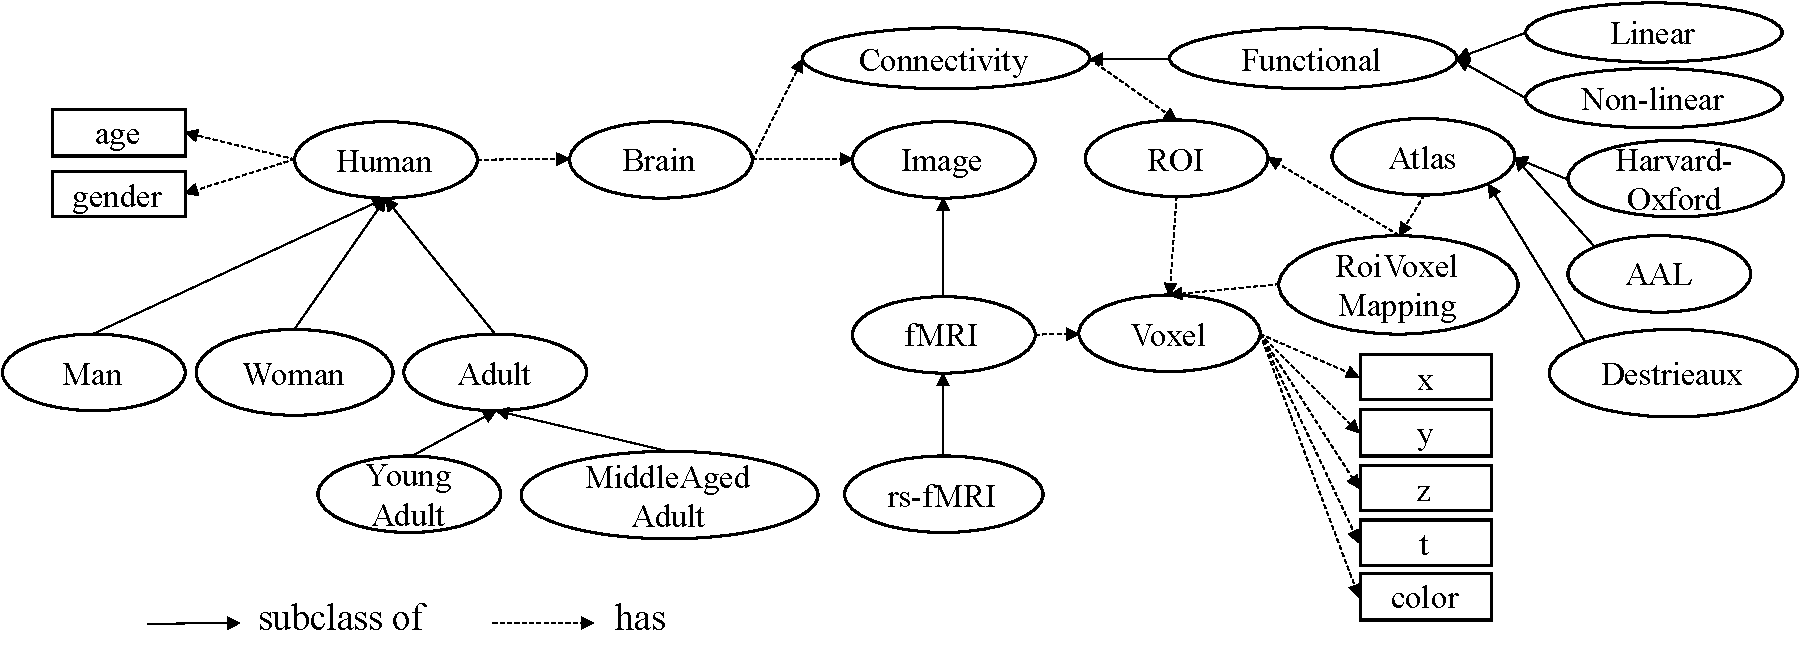
\includegraphics[width=1.0\linewidth]{images/DomainOnto.pdf}
    \caption{Воплощение гипотезы.}\label{fig:DomainOnto}
\end{figure}

Обычно онтологии предметной области могут быть намного больше по размеру и довольно сложны в эксплуатации. Преимущество их использования заключается в том, что они позволяют использовать движки логического вывода над ними. В онтологии предметной области есть основные понятия, такие как человек, мозг, изображение, атлас и т.д. Каждый класс является подклассом специального класса \textbf{Thing}. Простые свойства данных, такие как возраст, пол и пространственно-временные координаты, изображены в квадратах. OwlReady2 позволяет указать определение подкласса со следующей конструкцией, например, взрослый среднего возраста "--- это взрослый, возраст которого составляет от 30 до 45 лет, является подклассом взрослого (подкласс человека, где определяются возрастные и гендерные функциональные свойства) и не связан с классом \textbf{YoungAdult}:

\begin{ListingEnv}[!h]% настройки floating аналогичны окружению figure
    \captiondelim{ } % разделитель идентификатора с номером от наименования
    \caption{Часть онтологии предметной области с использованием OwlReady2}\label{lst:ontology}
    % окружение учитывает пробелы и табуляции и применяет их в сответсвии с настройками
    \begin{lstlisting}[language={Python}]
    
    class Human(Thing): pass
    class has_age(Human >> int, DataProperty, 
                    FunctionalProperty): pass
    class has_gender(Human >> int, DataProperty, 
                    FunctionalProperty): pass

    class Adult(Human):
            equivalent_to = [Human & has_age > 18]
    class YoungAdult(Adult):
            equivalent_to = [Adult & has_age < 30]
    class MiddleAgedAdult(Adult):
            equivalent_to = [Adult & has_age >= 30 & 
                            has_age < 45]
                            
    AllDisjoint([YoungAdult, MiddleAgedAdult])
\end{lstlisting}
\end{ListingEnv}

Нейроизображение "--- 4-мерное изображение (серия 3-мерных изображений), отражающее распределение метаболической активности в разных областях мозга в разные промежутки времени. Область мозга представляет собой набор вокселов, отсортированных по определенному признаку. Чаще всего представляется в виде временных рядов. Воксель - это элемент трехмерного изображения, содержащий некоторое значение.

Связность мозга "--- структура анатомических связей, статистических зависимостей или причинно-следственных взаимодействий между отдельными единицами нервной системы мозга. Структурная связность относится к сети физических или структурных связей, связывающих наборы нейронов или нейронных элементов со структурными биофизическими особенностями. Функциональная связность "--- это статистический тип связи между анатомически несвязанными областями мозга, которые обладают общими функциональными свойствами. Эффективная связность "--- сочетание структурной и функциональной связности. Она описывает сети направлений одного нейронного элемента по отношению к другому.

ФМРТ в состоянии покоя - это нейронное изображение, полученное в результате эксперимента, когда испытуемый находился в состоянии покоя и не занимался активными задачами.

\section{Спецификации гипотез и моделей для задач нейроинформатики}\label{sect_5_2}

Следующим шагом является определение гипотез предметной области, моделей и сопоставления гипотез с моделями. Есть четыре гипотезы, которые уточняются. Первый описывает, как следует выделять регионы головного мозга (ROI). Три конкурирующие модели, которые используют три атласа, сопоставлены с этой первой гипотезой. 

Вторая конкретизированная гипотеза касается функциональной связности и того, как ROI взаимодействуют друг с другом. Конкурирующие модели здесь линейные и нелинейные. Уравнения не указаны, и флаг для их генерации установлен в значение \textit{true}. 

Третья и четвертая гипотезы касаются существования значительных различий в функциональной связности у мужчин и женщин или у взрослых молодого и среднего возраста. Две конкурирующие модели для обеих гипотез "--- это модели разности уравнений и графов. Гипотезы и модели изображены на \cref{fig:Hypothesis_lattice}.

\begin{figure}[ht]
    \centering
    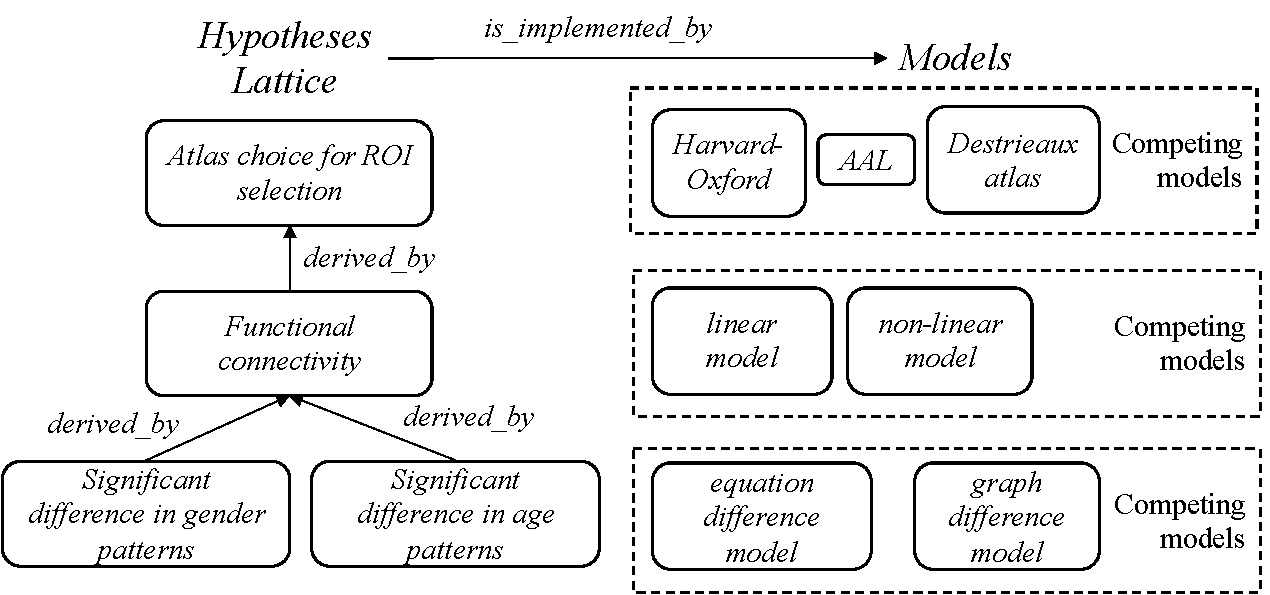
\includegraphics[width=1.0\linewidth]{images/Hypothesis_Lattice.pdf}
    \caption{Решетка гипотез для задач поиска различий в функциональной связности.}\label{fig:Hypothesis_lattice}
\end{figure}

Чтобы сгенерировать гипотезы на основе данных, требуется построить систему уравнений, описывающих функциональную взаимосвязь между несколькими переменными в наборе данных. Это не всегда необходимо в других областях, например, в астрономии теоретические уравнения известны заранее и их не нужно генерировать [10].
Для заявленной задачи нелинейные методы построения функциональных зависимостей позволяют построить большее количество моделей для более точного описания ожидаемых зависимостей [12]. Нелинейный подход заключается в построении нелинейной функции, которая выражает зависимость каждой отдельной переменной от других переменных. По умолчанию система использует генетическое программирование для построения нелинейных функций [13]. Это не требует каких-либо априорных предположений о зависимостях данных. Можно смешивать классы из онтологии домена с методами python. Для этого создается подкласс нелинейной модели из \textbf{Model} и добавляется метод \textit{fit} следующим образом:

\begin{ListingEnv}[!h]% настройки floating аналогичны окружению figure
    \captiondelim{ } % разделитель идентификатора с номером от наименования
    \caption{Определение нелинейной модели и ее метода \textit{fit}}\label{lst:fit}
    % окружение учитывает пробелы и табуляции и применяет их в сответсвии с настройками
    \begin{lstlisting}[language={Python}]
class NonLinearModel(Model):
    namespace = virtual_experiment_onto.
        get_namespace("http://synthesis.ipi.ac.ru/virtual_experiment.owl")

    def fit(self, X, y):
        est_gp = SymbolicRegressor(population_size=1000,
                                   tournament_size=20,
                                   generations=150, 
                                   stopping_criteria=0.001,
                                   const_range=(-1, 1),
                                   p_crossover=0.7, 
                                   p_subtree_mutation=0.12,
                                   p_hoist_mutation=0.06, 
                                   p_point_mutation=0.12,
                                   p_point_replace=1,
                                   init_depth=(6, 10),
                                   function_set=('mul', 'sub', 
                                         'div', 'add', 'cos'),
                                   max_samples=0.9,
                                   verbose=1,
                                   metric='mse',
                                   parsimony_coefficient=.005,
                                   random_state=0)

        est_gp.fit(X, y)
        return est_gp
\end{lstlisting}
\end{ListingEnv}

Подход к созданию моделей на основе данных использует общий метод линейной модели, основанный на данных. В результате таких комбинаций выбираются переменные, коэффициент для которых существенно отличается от нуля. Одновременно с общей линейной моделью для того же набора данных выполняется динамическое причинно-следственное моделирование. Комбинации выбранных переменных используются в качестве входных данных для метода генетического программирования. Использование такой эвристики может значительно сократить время работы генетического программирования, одновременно повышая точность соответствия данным наблюдений. Выходные системы уравнений ранжируются с использованием коэффициента детерминации; функция с наивысшим показателем возвращается эксперту.

\section{Сравнение конкурирующих гипотез для задачи поиска разности в образцах функциональной связности у мужчин и женщин}

Результаты сравнения различных гипотез и соответствующих им моделей приводится для задачи поиска различий в функциональной связности у мужчин и женщин в состоянии покоя. Постановка и описание задачи приведены в \cref{sect_4_1}. Для поставленной задачи были сформулированы гипотезы и реализующие их модели (см.\cref{fig:Hypothesis_lattice}). Слева приведен граф зависимости нескольких гипотез между собой. Вершиной графа является набор конкурирующих между собой гипотез. Конкурирующими являются гипотезы, описывающие один и тот же феномен и реали-зованные различными вычислительными моделями. Приведенные методы сравнения работают для конкурирующих гипотез, для зависимых гипотез они не применимы.

Система поддержки виртуальных экспериментов автоматически вычисляет множество экспериментов, сочетающих разные конкурирующие гипотезы. Проведено четыре виртуальных эксперимента (атлас выбирается вручную), с использованием двух типов моделей "--- линейных и нелинейных и двух типов разностей предсказаний.

Для данной задачи выделены три множества конкурирующих гипотез: вы-бор атласов и выделение регионов головного мозга человека, построение функ-циональной связности регионов головного мозга, поиск значимых различий в функциональной связности у мужчин и женщин в состоянии покоя. Для первого множества нет единого способа выбрать ту или иную модель. В работе \cite{Arslan2018} сравнивается множество различных методов для выделения регионов. Они сравнивают их по 4 критериям, а именно: воспроизводимость, сохранение информации в связи со значительным уменьшением размерности, интерпретируемость. При этом отмечается, что модели не полностью сравнимы, поэтому окончательный выбор остается за экспертом в зависимости от решаемой задачи, набора данных и необходимости сравнения с другими работами. 

Для второго множества конкурирующих гипотез о функциональной связности регионов головного мозга используется несколько методов. Первым шагом для данного сравнения является отсечение моделей по пороговому значению коэффициента детерминации. Это делается для сокращения пространства сравниваемых моделей. Для 23 построены модели с оценкой выше порогового коэффициента детерминации, равным 0.7. Вторым шагом является сравнение линейных и нелинейных моделей, где нелинейные модели бы-ли получены методом генетического программирования, пример которых представлен ниже:

\begin{equation}
\begin{array}{l}
x_0 = \frac{\left(x_{43}-x_{41}\right) * (x_{13}-x_{26} )}{x_{26}} + x_{41}-x_3 \\
x_1= x_{39} * (0.756-x_{40})    
\end{array}
\end{equation}

Для сравнения используется критерии Акаике и Байеса по причине возможности сравнения моделей различной природы. Результаты сравнения с использованием информационного критерия Акаике приведены в \cref{tbl:aic_bic_gender}. Здесь и далее результаты приводятся только для регионов \textit{Precentual Gyrus}, \textit{Postcentral Gyrus} и \textit{Planum Polare}. Для критерия Акаике лучшей моделью является нелинейная модель, то время, как для критерия Байеса лучшей моделью оказалась линейная модель.

\begin{table} [ht]%
	\caption{Результаты сравнения моделей по информационным критериям}%
	\label{tbl:aic_bic_gender}% label всегда желательно идти после caption
    \setlength\extrarowheight{0pt} %вот этим управляем расстоянием между рядами, \arraystretch даёт неудачный результат
    \setlength{\tymin}{2.3cm}% минимальная ширина столбца
    \begin{center}

	\begin{tabulary}{\textwidth}{@{}>{\zz}L >{\zz}C >{\zz}C >{\zz}C >{\zz}C@{}}% Вертикальные полосы не используются принципиально, как и лишние горизонтальные (допускается по ГОСТ 2.105 пункт 4.4.5) % @{} позволяет прижиматься к краям
        \toprule     %%% верхняя линейка
    	  Регион &
    	AIC (линейная) &
            AIC (ГП) &
            BIC (линейная) &
            BIC (ГП) 
            \\
        \midrule %%% тонкий разделитель. Отделяет названия столбцов. Обязателен по ГОСТ 2.105 пункт 4.4.5 
        \textit{Precentual Gyrus} &
        -53\,058 &
        -58\,638 & 
        -54\,987 &
        -37\,821
        \\
        \midrule
        \textit{Postcentral Gyrus} &
        -46\,048 &
        -52\,315 & 
        -42\,874 &
        -34\,508  
        \\
        \midrule
        \textit{Planum Polare} &
        -7\,109 &
        -10\,658 & 
        -6\,925 &
        -3\,215    
        \\
        \bottomrule %%% нижняя линейка
	\end{tabulary}%
 \end{center}

\end{table}



Несоответствие между двумя информационными критериями вызвано тем, что в критерии Байеса учитывается не только точность предсказания, но также и сложность проверяемой модели. В модели генетического программирования число параметров значительно больше, чем в обычной линейной модели, поэтому у критерия Байеса оценка модели генетического программирования больше, чем у линейной. Если требуется не только точность предсказаний, но и простота модели, то следует использовать критерий Байеса, иначе критерий Акаике.

Третье множество конкурирующих гипотез о поиске значимых различий в функциональной связности у мужчин и женщин в состоянии покоя состоит из двух конкурирующих гипотез. Каждая из гипотез реализована следующими мо-делями. Первая модель представляет собой разность между предсказаниями для мужчин и женщин в выбранном регионе. Вторая модель строится вычитанием графов, построенных для мужчин и женщин, каждый из которых описывает взаимодействие между регионами головного мозга. Данные гипотезы не являются сравнимыми напрямую, а скорее являются взаимодополняющими. Если полу-ченные регионы со значимыми различиями не совпадают, то эксперту рекомендуется дополнительно проверить данный регион, например, используя другой набор данных.

Для первой модели проверяется равность медианы разности нулю с использованием статистического теста "--- критерия знаков \cite{pham2019new}, а также байесовского подхода. Результаты представлены в \cref{tbl:gp_2datasets} для трех регионов без потери наглядности.

\begin{table} [ht]%
	\caption{Результаты сравнения двух моделей генетического программирования, обученных на разных выборках}%
	\label{tbl:gp_2datasets}% label всегда желательно идти после caption
    \setlength\extrarowheight{0pt} %вот этим управляем расстоянием между рядами, \arraystretch даёт неудачный результат
    \setlength{\tymin}{2.3cm}% минимальная ширина столбца
    \begin{center}

	\begin{tabulary}{\textwidth}{@{}>{\zz}L >{\zz}C@{}}% Вертикальные полосы не используются принципиально, как и лишние горизонтальные (допускается по ГОСТ 2.105 пункт 4.4.5) % @{} позволяет прижиматься к краям
        \toprule     %%% верхняя линейка
    	  Регион &
    	Достигаемый уровень значимости 	\\
        \midrule %%% тонкий разделитель. Отделяет названия столбцов. Обязателен по ГОСТ 2.105 пункт 4.4.5 
        \textit{Precentual Gyrus} &
        0.0045 (отвергается) 
        \\
        \midrule
        \textit{Postcentral Gyrus} &
        0.0003 (отвергается)  
        \\
        \midrule
        \textit{Planum Polare} &
        0.08 (не отвергается)  
        \\
        \bottomrule %%% нижняя линейка
	\end{tabulary}%
 \end{center}

\end{table}

Уровень значимость выбран равным 0.05. Регионы \textit{Precentual Gyrus} и \textit{Postcentral Gyrus} являются различными для мужчин и женщин.  Для региона \textit{Planum Polare} нулевая гипотеза о схожести регионов не отвергается. Важным замечанием является то, что хотя нулевая гипотеза не отвергается, но полученное значение близко к порогу 0.05. Если выбрано значение порога, например, 0.1, то нулевая гипотеза о схожести региона отвергается для \textit{Planum Polare}. 

Результаты сравнения для байесовского подхода представлены в \cref{tbl:bayesian_gender}. Результаты совпадают с результатами для статистического теста. При этом появляется возможность оценить степень уверенности в результате. 

\begin{table} [ht]%
	\caption{Результаты сравнения байесовским подходом}%
	\label{tbl:bayesian_gender}% label всегда желательно идти после caption
    \setlength\extrarowheight{0pt} %вот этим управляем расстоянием между рядами, \arraystretch даёт неудачный результат
    \setlength{\tymin}{2.3cm}% минимальная ширина столбца
    \begin{center}

	\begin{tabulary}{\textwidth}{@{}>{\zz}L >{\zz}L >{\zz}C@{}}% Вертикальные полосы не используются принципиально, как и лишние горизонтальные (допускается по ГОСТ 2.105 пункт 4.4.5) % @{} позволяет прижиматься к краям
        \toprule     %%% верхняя линейка
    	  Регион &
            $\eta$ &
    	Доказательная сила 	\\
        \midrule %%% тонкий разделитель. Отделяет названия столбцов. Обязателен по ГОСТ 2.105 пункт 4.4.5 
        \textit{Precentual Gyrus} &
        $29:1 (29)$ &
        Среднее доказательство 
        \\
        \midrule
        \textit{Postcentral Gyrus} &
        $54:1 (54)$ &
        Среднее доказательство  
        \\
        \midrule
        \textit{Planum Polare} &
        $7:1 (0.14)$ &
        Слабое доказательство
        \\
        \bottomrule %%% нижняя линейка
	\end{tabulary}%
 \end{center}

\end{table}

Для \textit{Precentual Gyrus} и \textit{Postcentral Gyrus} нулевая гипотеза схожести этих регионов у мужчин и женщин отвергается со средней степенью уверенности. При этом для \textit{Planum Polare} нулевая гипотеза не отвергается со слабой степенью уверенности, что говорит о необходимости дополнительного исследования данного региона. В целом результаты статистического и байесовского подхода схожи, но иногда они могут давать различные результаты. Для трех регионов было получено, что при использовании статистического теста регионы получились различны.

Другой предлагаемый метод сравнения гипотез основан поиска схожести графового представления соответствующих им моделей. На вход метод принимает теоретическую гипотезу в виде системы уравнений и набор данных, по которому будут сгенерированы конкурирующие гипотезы. По данным автоматически генерируются несколько конкурирующих гипотез. Производится вычисление для всех сгенерированных моделей выбранной экспертом метрики, отбирается одна лучшая гипотеза. Для обеих моделей, реализующих гипотезы (теоретическая гипотеза "--- построенная из данных гипотеза), строятся ориентированные ацикличные графы зависимости переменных из уравнений. Далее для пары графов выполняется сравнение их сходства посредством построения графа разности. Если для построенного графа его множество ребер не является пустым, то гипотезы считаются различными и возвращается истина, иначе возвращается ложь. Метод может быть применен, если модели представимы в виде ацикличных графов.

В качестве примера строится разность двух графов для мужчин и женщин \cref{fig:graph_difference}. Вершинами построенного графа разности являются регионы мозга, а ребрами – связи между регионами. Если функциональная связность региона является раз-личной у мужчин и женщин, то в графе разности присутствует хотя бы одно ребро для данного региона. Для полученного графа видно, что для регионов \textit{Postcentral Gyrus} и \textit{Planum Polare} получился такой же результат, как и в случае с использованием первой модели. Для региона \textit{Precentual Gyrus} результат отличается, т.~е. эксперту рекомендуется провести дополнительные исследования.


\begin{figure}[ht]
    \centering
    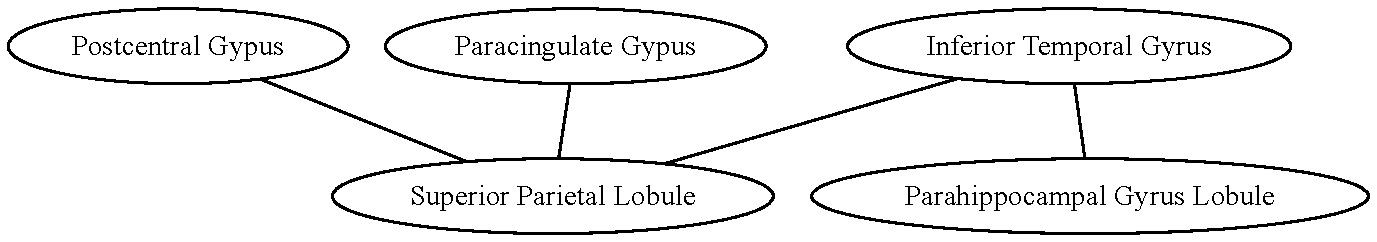
\includegraphics[width=1.0\linewidth]{images/graph_difference.pdf}
    \caption{Граф разности функциональной связности регионов для мужчин и женщин.}\label{fig:graph_difference}
\end{figure}

\section{Построение решетки гипотез}\label{sect_5_3}
Для работы с набором гипотез используется концепция решетки гипотез \cref{sect2_3}. Решетка используется для анализа того, какие части виртуального эксперимента необходимо пересчитать, а какие части можно загрузить из репозитория. Поток работ и его отображение в модели, реализованные на Python, изображены на \cref{fig:workflow}.

\begin{figure}[ht]
    \centering
    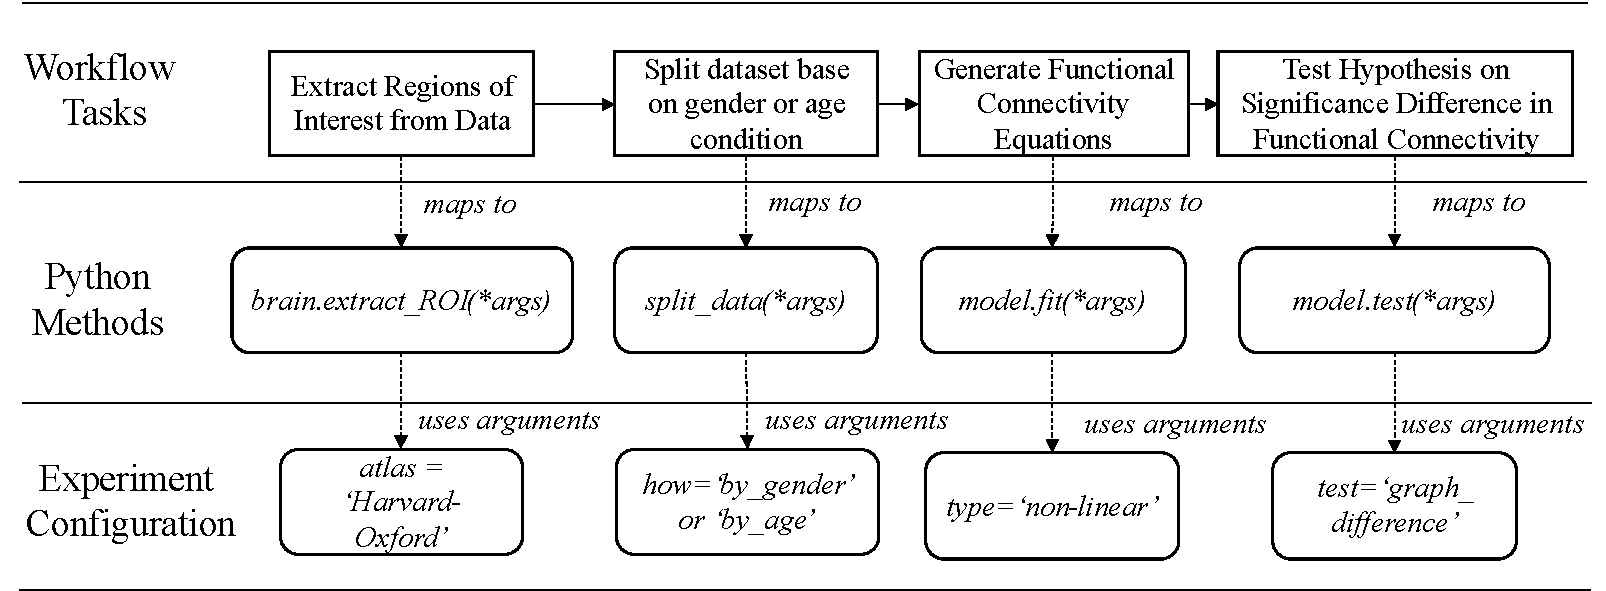
\includegraphics[width=1.0\linewidth]{images/Workflow_conf.pdf}
    \caption{Поток работ и конфигурация.}\label{fig:workflow}
\end{figure}

Параметры модели описаны в конфигурации. Извлечение ROI является общим шагом для обеих проблем. На этом этапе требуется преобразовать 4-мерное изображение мозга в двумерный массив (области мозга - время). Интересующие регионы группируются и усредняются некоторым образом, и само среднее значение является репрезентативным значением для данного региона. Самый популярный способ "--- использовать карты мозга - атласы. При работе с атласами человеческого мозга используется предварительно рассчитанная функция, которая присваивает каждому вокселу изображения некоторую область мозга.
Следующая задача потока работ "--- разделить набор данных по полу или возрасту. Выбор делается на основе конфигурации виртуального эксперимента. Третья задача "--- сгенерировать уравнения функциональной связности. Здесь могут быть использованы линейные и нелинейные модели. Эта задача реализуется компонентом генерации. Последняя задача "--- проверить гипотезу о наличии существенной разницы для обученных моделей.



\clearpage